\section{Data}\label{subsec:data}
\francis{\em This section is under construction}
Cryptocurrenices are traded around the clock, but CME future are traded from
Sunday to Friday from 05:00 p.m. to 04:00 p.m. U.S. central time.
We match the timestamps and timezones of different data sources.


\begin{table}[htbp]
    \centering
    \begin{tabularx}{\textwidth}{s|CCCCCCCC}
      \hline\hline
     \# & Asset & Data Source & Type & Tradable at CT\footnotemark & Tradable at CET\footnotemark during CST\footnotemark & Tradable at CET during CDT\footnotemark & Tradable at UTC during CST & Tradable at UTC during CDT\\       \hline
      1 & Bitcoin & Coingecko API & Hourly Close &  & 11:00pm D+0 & 11:00pm D+0 & 10:00pm D+0$^*$ &10:00pm D+0$^*$ \\\hline
      2 & CME Future & Bloomberg & Daily Open & 05:00pm D-1 & 00:00am D+0$^*$ & 00:00am D+0$^*$ & 11:00pm D-1 & 10:00pm D-1 \\       \hline
      3 & CME Future & Bloomberg & Daily Close & 04:00pm D+0& 11:00pm D+0$^*$ & 11:00pm D+0$^*$ & 10:00pm D+0 & 09:00pm D+0\\       \hline
      4 & CRIX & IRTG (from Coingecko) & Index &  &  &  & & 00:00am D+0$^*$\\\hline
    \end{tabularx}
    \caption{$^*$ indicates the timestamp of raw data from data source. }
    \label{tab:table}
\end{table}

\addtocounter{footnote}{-3}
\footnotetext{CT stands for U.S. Central Time. It represents two observances of time, the Central Standard Time (CST) and the Central Daylight Time (CDT)}
\addtocounter{footnote}{1}
\footnotetext{CET stands for Central European Time. It is one hour ahead UTC.}
\addtocounter{footnote}{1}
\footnotetext{CST is six hours behind UTC.}
\addtocounter{footnote}{1}
\footnotetext{CDT is five hours behind UTC.}

Hedging Pair 1 is hedging \#1 (Bitcoin Spot) with \#3 (CME future).
The time difference between the two prices is zero.
They are both adjusted to CET time:
\#1 by pandas.Series.dt.tz\_convert; \#3 by retrieving data from Bloomberg Terminal located in Berlin. \medskip

Hedging Pair 2 is hedging \#4 (CRIX) with \#2 (CME future).
We observe \#2 two hours and one hour before \#4 during CST and CDT respectively.


\subsection{Time Difference}\label{subsec:time-difference}
\begin{table}[h]
    \centering

\begin{tabular}{lrrrr}
\toprule
{} &     Open &     High &      Low &    Close \\
\midrule
2021-02-02 23:00 &  36360.0 &  38155.0 &  36240.0 &  37790.0 \\
2021-02-01 23:00 &  34205.0 &  36665.0 &  34070.0 &  36535.0 \\
2021-01-31 23:00 &  33715.0 &  35280.0 &  32800.0 &  34265.0 \\
2021-01-28 23:00 &  33995.0 &  39530.0 &  32590.0 &  35180.0 \\
2021-01-27 23:00 &  31005.0 &  33710.0 &  30350.0 &  33085.0 \\
\bottomrule
\end{tabular}
       \caption{CME Bitcoin Future Raw Data}
    \label{tab:table0} \medskip

    \begin{tabular}[width=\textwidth]{llrrrr}
\toprule
 &                      date &           CRIX &   future &  log return CRIX &  log return future \\
\midrule
0 & 2021-02-04  &  104518.468839 &  38080.0 &         0.054757 &           0.046220 \\
1 & 2021-02-03  &   98949.179255 &  36360.0 &         0.059741 &           0.061097 \\
2 & 2021-02-02  &   93210.948461 &  34205.0 &         0.002204 &           0.014429 \\
3 & 2021-02-01  &   93005.711051 &  33715.0 &         0.013628 &          -0.008271 \\
4 & 2021-01-29  &   91746.863103 &  33995.0 &         0.081917 &           0.092065 \\
\bottomrule
    \end{tabular}
    \caption{CRIX \#4 with Opening price of CME Bitcoin future \#2 and their log returns}
    \label{tab:table2} \medskip

\begin{tabular}{llrrrr}
\toprule
{} &                      date &           CRIX &   future &  log return CRIX &  log return future \\
\midrule
0 & 2021-02-05  &  103348.488555 &  38220.0 &        -0.011257 &           0.011314 \\
1 & 2021-02-04  &  104518.468839 &  37790.0 &         0.054757 &           0.033774 \\
2 & 2021-02-03  &   98949.179255 &  36535.0 &         0.059741 &           0.064146 \\
3 & 2021-02-02  &   93210.948461 &  34265.0 &        -0.016175 &          -0.026353 \\
4 & 2021-01-30  &   94730.919657 &  35180.0 &         0.032007 &           0.061398 \\
\bottomrule
\end{tabular}
    \caption{CRIX \#4 with Closing price of CME Bitcoin future \#3 shifted for one day (D-1) and their log returns}
    \label{tab:table3}
\end{table}

\clearpage
\begin{figure}[ht]
    \centering
    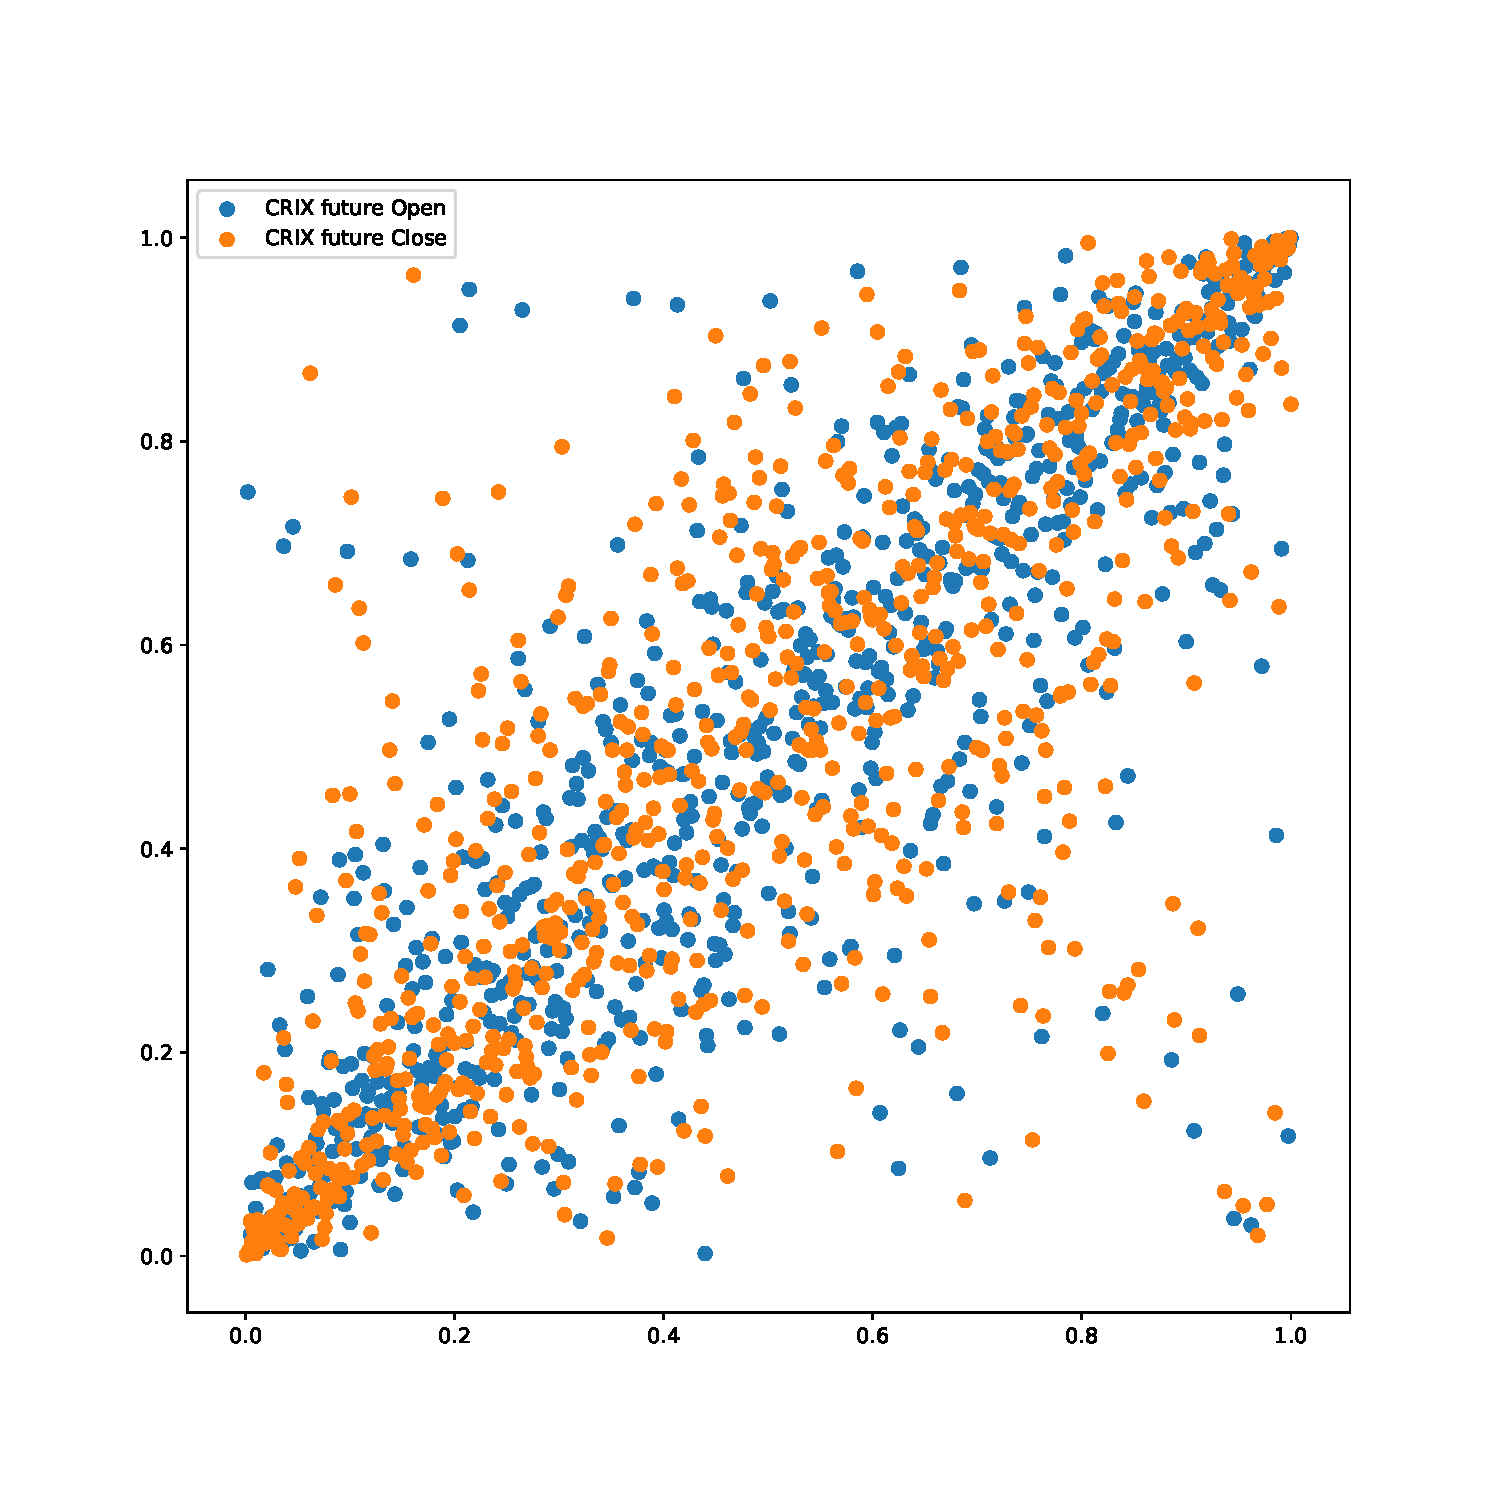
\includegraphics[scale=.35]{_pics_notes/CRIX_future_Open_Close.pdf}
    \end{figure}

Kendall's tau between CRIX and future Close is 0.608429;\\
Kendall's tau between CRIX and future Open is 0.673266; we pick this unless we have hourly CRIX.

\subsection{Statistics of Percentage Difference Between CME Bitcoin future Open Price and Last Close Price}

$$\text{diff} = \frac{\text{Open}_{t} - \text{Close}_{t-1}} {\text{Close}_{t-1}}$$

Mean of diff = 0.00236\\
Std of diff = 0.02206\\
Max of diff = 0.16394 \\
UQ of diff = 0.00814 \\
Median of diff = 0.00132\\
LQ of diff = -0.00412 \\
Min of diff = -0.12190 \\
